\documentclass[12pt]{article}

% ------------------ Fuentes e idioma ------------------
\usepackage{fontspec}
\usepackage{polyglossia}
\setmainlanguage{spanish}

% ------------------ Márgenes ------------------
\usepackage[margin=2.5cm]{geometry}

% ------------------ Matemáticas ------------------
\usepackage{amsmath}
\usepackage{amssymb}
\usepackage{amsthm}

% ------------------ Tablas ------------------
\usepackage{booktabs}
\usepackage{array}
\usepackage{longtable}

% Corrige un conflicto de booktabs+longtable con polyglossia (español) que
% causa "Undefined control sequence \cmrsideswitch" en tablas largas: fuerza
% las reglas (\toprule, \midrule, \bottomrule) a usar el modo simple en vez
% del modo optimizado para longtable, que es el que dispara el bug.
\makeatletter
\def\@BTrule[#1]{%
  \let\@BTswitch\@BTnormal
  \global\@thisrulewidth=#1\relax
  \ifnum\@thisruleclass=\tw@\vskip\@aboverulesep\else
  \ifnum\@lastruleclass=\z@\vskip\@aboverulesep\else
  \ifnum\@lastruleclass=\@ne\vskip\doublerulesep\fi\fi\fi
  \@BTswitch}
\makeatother

% ------------------ Gráficas ------------------
\usepackage{graphicx}
\graphicspath{{figures/}}

% ------------------ Hipervínculos ------------------
\usepackage{hyperref}
\hypersetup{
    colorlinks=true,
    linkcolor=blue,
    citecolor=blue,
    urlcolor=blue
}

% ------------------ Datos de portada ------------------
\title{Tarea 1 \\ \large Inferencia Causal}
\author{Jhonatan Román Román}
\date{22 de septiembre de 2026}

\begin{document}

\maketitle

\section{Pregunta 1}

\textit{Los datos en data-salud.csv contienen los registros de 915 pacientes que participaron en un ensayo clínico en el que se trabaja con $\alpha = 0.10$. Se incluye un índice de salud que resume la calidad de la salud de cada paciente (a mayor índice de salud mejor es la salud), así como 10 características observadas de dichas personas. Un cuarto de los pacientes fue asignado aleatoriamente a un tratamiento identificado como $D$ en los datos.}

\subsection*{Inciso (a)}

\textit{[5 puntos] Para verificar la integridad del diseño, compruebe que cada una de las características observables está balanceada. Para ello, estime una regresión de cada una de las características en función de la variable de tratamiento. Construya una tabla con los coeficientes de interés estimados y el valor p correspondiente.}

Para cada característica observable se estima:
\begin{equation}
X_k = \alpha + \beta_1 D + \epsilon
\end{equation}
donde $X_k$ es la $k$-ésima característica observable, $D$ es la variable de tratamiento y $\epsilon$ es el término de error.


\begin{longtable}[t]{lrrrl}
\caption{Balance de covariables entre grupos de tratamiento}\\
\toprule
Característica & Coeficiente & Error estándar & Valor p & Balanceada\\
\midrule
edad & 0.088 & 0.938 & 0.925 & TRUE\\
ingreso & -561.401 & 653.796 & 0.391 & TRUE\\
educacion & -0.312 & 0.226 & 0.169 & TRUE\\
imc & 0.208 & 0.317 & 0.512 & TRUE\\
fumador & 0.036 & 0.033 & 0.272 & TRUE\\
ejercicio & 0.036 & 0.038 & 0.341 & TRUE\\
cronica & -0.048 & 0.031 & 0.121 & TRUE\\
seguro & 0.011 & 0.037 & 0.771 & TRUE\\
urbano & -0.026 & 0.036 & 0.471 & TRUE\\
mujer & -0.037 & 0.038 & 0.331 & TRUE\\
\bottomrule
\end{longtable}



\subsection*{Inciso (b)}

\textit{[2 puntos] ¿Cuál es la hipótesis nula que se plantea al realizar cada una de las regresiones en la parte a.?}

La hipótesis nula en cada regresión es que el coeficiente de $D$ es igual a cero, es decir, que no existe diferencia en la media de la característica observable entre el grupo tratado y el grupo de control:
\[
H_0: \beta_1 = 0
\]

\subsection*{Inciso (c)}

\textit{[2 puntos] ¿Qué concluye a partir de las estimaciones de la parte a.?}

El valor p del coeficiente de $D$ es mayor a $0.10$ en las diez regresiones, así que no se rechaza $H_0$ en ningún caso. Los grupos tratado y control están balanceados en todas las covariables observables. Esto es consistente con una asignación aleatoria del tratamiento.

\subsection*{Inciso (d)}

\textit{[3 puntos] Pruebe de manera conjunta si las características observables predicen la asignación al tratamiento. Para ello, estime una regresión de $D$ en función de las 10 características observables y realice una prueba F de significancia conjunta.}

Se estima:
\begin{equation}
D = \alpha + \beta_1 X_1 + \beta_2 X_2 + \dots + \beta_{10} X_{10} + \epsilon
\end{equation}
donde cada $X_k$ es una de las diez características observables.

La hipótesis nula de la prueba F es:
\[
H_0: \beta_1 = \beta_2 = \dots = \beta_{10} = 0
\]


\begin{longtable}[t]{rlr}
\caption{Prueba F de significancia conjunta}\\
\toprule
Estadístico F & Grados de libertad & Valor p\\
\midrule
0.9199 & 10, 904 & 0.5139\\
\bottomrule
\end{longtable}


\subsection*{Inciso (e)}

\textit{[2 puntos] ¿Cuál es la hipótesis nula de la prueba F que realizó en la parte d.?}

La hipótesis nula es que todos los coeficientes de las características observables son simultáneamente iguales a cero, es decir, ninguna covariable predice la asignación al tratamiento:
\[
H_0: \beta_1 = \beta_2 = \dots = \beta_{10} = 0
\]

\subsection*{Inciso (f)}

\textit{[2 puntos] ¿Qué concluye a partir de la prueba F de la parte d.?}

El estadístico F es $0.9199$ con valor p $= 0.5139$, mayor a $0.10$, así que no se rechaza $H_0$. El tratamiento no está relacionado con las covariables observables en conjunto.

\subsection*{Inciso (g)}

\textit{[2 puntos] ¿Qué concluye sobre el balance en la asignación del tratamiento en este experimento? ¿Qué características tendría una diferencia de medias de $y_i$ después del tratamiento como estimador del impacto de este?}

Los resultados de (a) y (d) muestran que ninguna covariable predice el tratamiento y que los grupos son estadísticamente equivalentes en todas las características observables. Esto confirma que la asignación fue aleatoria.

Dado el balance, una diferencia de medias de $Y$ entre tratados y controles es un estimador insesgado del efecto promedio del tratamiento (ATE). La aleatorización garantiza que los grupos son comparables en expectativa tanto en características observables como no observables.

\section{Pregunta 2}

\textit{Usando los mismos datos de data-salud.csv, estime el efecto del tratamiento $D$ sobre el índice de salud $Y$, primero sin controles y luego incorporando las características observables.}

\subsection*{Inciso (a)}

\textit{[2 puntos] Estime el efecto del tratamiento sobre el índice de salud usando una regresión corta (sin controles).}

Se estima:
\begin{equation}
Y_i = \alpha + \beta D_i + \epsilon_i
\end{equation}


\begin{longtable}[t]{lrrlr}
\caption{Regresión corta: efecto del tratamiento sobre Y}\\
\toprule
Término & Coeficiente & Error estándar & Valor p & R2\\
\midrule
Intercepto & 55.5092 & 0.5095 & 0.00e+00 & 0.0531\\
D & 7.2856 & 1.0184 & 1.73e-12 & NA\\
\bottomrule
\end{longtable}


El coeficiente de $D$ es $7.2856$ (error estándar $1.0184$, p $< 0.001$). El efecto del tratamiento es positivo sobre el índice de salud.

\subsection*{Inciso (b)}

\textit{[3 puntos] Interprete el coeficiente y la significancia estadística del efecto de tratamiento estimado.}

El coeficiente de $D$ indica que los pacientes tratados tienen, en promedio, un índice de salud $7.2856$ puntos mayor que los no tratados. El valor p ($1.73\text{e-}12$) es mucho menor a $\alpha = 0.10$, así que se rechaza $H_0: \beta = 0$. El efecto del tratamiento es estadísticamente significativo y positivo sobre la salud.

\subsection*{Inciso (c)}

\textit{[2 puntos] Estime ahora el efecto del tratamiento sobre el índice de salud usando una regresión larga (incluyendo controles).}

Se estima:
\begin{equation}
Y_i = \alpha + \beta D_i + \sum_{k=1}^{10} \gamma_k X_{ki} + \epsilon_i
\end{equation}


\begin{longtable}[t]{lrrl}
\caption{Regresión larga: efecto del tratamiento sobre Y con controles}\\
\toprule
Término & Coeficiente & Error estándar & Valor p\\
\midrule
(Intercept) & 75.7572 & 1.7280 & 7.22e-226\\
D & 7.4853 & 0.4414 & 3.26e-56\\
edad & -0.3131 & 0.0156 & 2.22e-74\\
ingreso & 0.0003 & 0.0000 & 8.94e-46\\
educacion & 1.3165 & 0.0645 & 1.63e-76\\
imc & -1.1200 & 0.0460 & 4.25e-101\\
fumador & -9.7105 & 0.4444 & 2.70e-85\\
ejercicio & 9.3177 & 0.3885 & 1.00e-98\\
cronica & -14.6787 & 0.4689 & 3.07e-146\\
seguro & 4.3091 & 0.3951 & 4.26e-26\\
urbano & 1.9012 & 0.4092 & 3.89e-06\\
mujer & 0.8482 & 0.3831 & 2.71e-02\\
\bottomrule
\end{longtable}


El coeficiente de $D$ es $7.4853$ (error estándar $0.4414$, p $= 3.26\text{e-}56$). El efecto sigue siendo positivo y estadísticamente significativo al incluir controles.

\subsection*{Inciso (d)}

\textit{[3 puntos] Explique qué pasa y por qué con el error estándar estimado del efecto de tratamiento con respecto al estimado en la parte a.}

El error estándar de $D$ baja de $1.0184$ en la regresión corta a $0.4414$ en la larga. Los controles explican gran parte de la variación de $Y$ (el $R^2$ pasa de $0.053$ a $0.826$), lo que reduce la varianza del error y con ella el error estándar del estimador. El coeficiente de $D$ casi no cambia porque, al estar el tratamiento balanceado, no está correlacionado con los controles.

\section{Pregunta 3}

\textit{Un grupo de investigadores está interesado en conocer el impacto de la adopción de herramientas de inteligencia artificial en el empleo en pequeñas y medianas empresas del sector industrial, $y_i$. Para responder esta pregunta, los investigadores levantan una encuesta representativa de empresas pequeñas y medianas del sector industrial donde se pregunta sobre el uso de inteligencia artificial en los distintos procesos. Los investigadores construyen un indicador del uso de inteligencia artificial, $T_i$, además de recolectar información sobre el uso de insumos, ingresos, costos y número de empleados.}

\subsection*{Inciso (a)}

\textit{[5 puntos] Se propone que, para estimar el efecto causal del uso de inteligencia artificial sobre el empleo, se compare el número de empleados en las empresas que usan dicha tecnología con las que no la utilizan. Argumente en términos del sesgo de selección sobre la conveniencia de esta estrategia para estimar el efecto causal de la adopción de herramientas de inteligencia artificial.}

La comparación simple está sesgada porque la adopción de IA no es aleatoria. Las empresas que adoptan IA son sistemáticamente distintas de las que no lo hacen (mayor capital, mejor gestión, más recursos), así que la diferencia en empleo refleja tanto el efecto del tratamiento como estas diferencias preexistentes. Formalmente, existe sesgo de selección porque
\[
E[y_i(0) \mid T_i = 1] \neq E[y_i(0) \mid T_i = 0].
\]
La comparación simple no aísla el efecto causal.

\subsection*{Inciso (b)}

\textit{[5 puntos] Para implementar la propuesta del punto a., se propone estimar la siguiente regresión: $y_i = \alpha + \beta T_i + \varepsilon_i$. Muestre si el estimador de MCO de $\beta$ es consistente o no para el efecto de tratamiento.}

El estimador de MCO converge en probabilidad a:
\[
\hat{\beta} \xrightarrow{p} \beta + \frac{\text{Cov}(T_i, \varepsilon_i)}{\text{Var}(T_i)}.
\]
El estimador es consistente solo si $\text{Cov}(T_i, \varepsilon_i) = 0$. Por el sesgo de selección del inciso (a), $T_i$ está correlacionado con $\varepsilon_i$, así que $\text{Cov}(T_i, \varepsilon_i) \neq 0$. Por lo tanto $\hat{\beta}$ es inconsistente para el efecto causal de $T_i$.

\section{Pregunta 4}

\textit{Usando la Encuesta Nacional de Ocupación y Empleo (ENOE) 2023, se busca estimar la relación entre los años de escolaridad y el ingreso laboral usando la función esperanza condicional (FEC).}

\subsection*{Inciso (a)}

Se utiliza la ENOE 2023, una encuesta representativa a nivel nacional de México levantada por el INEGI. La muestra se restringe a la población ocupada (\texttt{clase2 == 1}) con ingreso mensual y horas trabajadas positivas, y años de escolaridad entre 0 y 25. Se excluyen observaciones con \texttt{anios\_esc > 25} porque en la ENOE esos valores corresponden a códigos especiales de no respuesta o no especificado, no a años reales de escolaridad. Además, se excluye el 1\% superior e inferior de la distribución del log del ingreso semanal para evitar que valores extremos distorsionen las estimaciones. La muestra final queda con $125{,}132$ observaciones.

\subsection*{Inciso (b)}

\textit{Estime la función esperanza condicional del log del ingreso semanal dado los años de escolaridad, primero con los microdatos y luego con las medias condicionales por año de escolaridad ponderadas por su frecuencia. Compare los coeficientes obtenidos.}

Regresión con microdatos:
\begin{equation}
Y_i = \alpha + \beta S_i + \epsilon_i
\end{equation}
donde $Y_i$ es el logaritmo del ingreso semanal y $S_i$ son los años de escolaridad del individuo $i$.

Regresión sobre las medias condicionales por año de escolaridad, ponderada por el número de observaciones $n_e$ en cada grupo:
\begin{equation}
\overline{Y}_e = \alpha + \beta S_e + u_e, \quad \text{ponderado por } n_e
\end{equation}
donde $\overline{Y}_e$ es la media condicional de $Y_i$ para el grupo con $S_e$ años de escolaridad.


\begin{longtable}[t]{lrrrr}
\caption{Comparación: regresión con microdatos vs. regresión sobre medias condicionales (FEC)}\\
\toprule
Regresión & Intercepto & Coeficiente años esc. & Error estándar & N\\
\midrule
Microdatos & 6.7847 & 0.0588 & 0.0004 & 125132\\
Medias ponderadas & 6.7847 & 0.0588 & 0.0034 & 25\\
\bottomrule
\end{longtable}


Los coeficientes de años de escolaridad son idénticos en ambas regresiones ($0.0588$), al igual que el intercepto ($6.7847$). Esto es consistente con el teorema de la FEC: la regresión lineal ponderada sobre las medias condicionales replica exactamente los coeficientes de la regresión con microdatos, ya que la FEC es la mejor aproximación lineal a la esperanza condicional muestral.

\subsection*{Inciso (c)}

\textit{Realice una figura análoga a la figura 3.1.1 en MHE, usando los datos que construyó para esta pregunta.}

\begin{figure}[h]
\centering
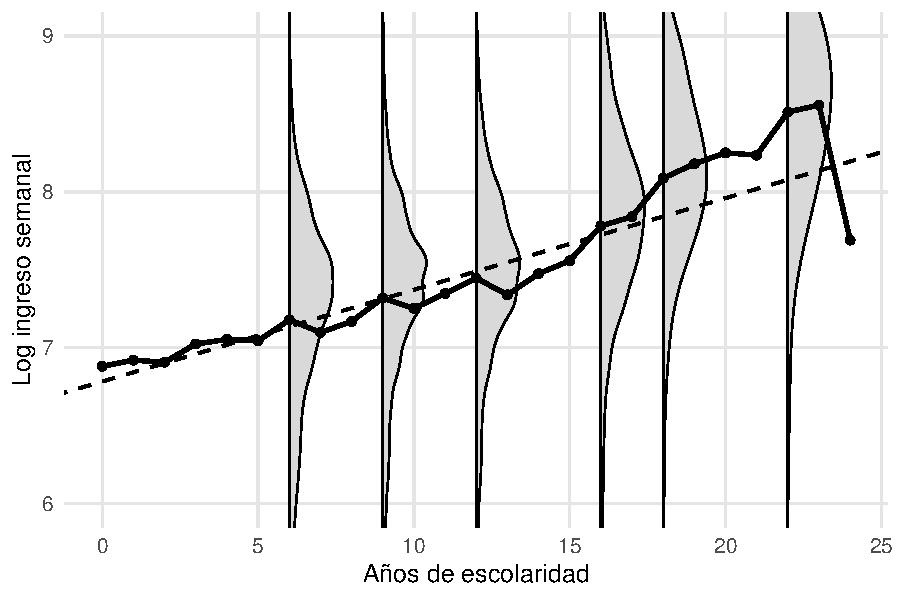
\includegraphics[width=0.8\textwidth]{figures/figura_fec.pdf}
\caption{Función esperanza condicional muestral del log del ingreso semanal dado los años de escolaridad. Los puntos negros conectados son las medias condicionales por año de escolaridad; la línea discontinua es la regresión lineal con microdatos. Las curvas verticales muestran la distribución condicional del log del ingreso semanal en los niveles educativos clave de México: primaria completa (6 años), secundaria completa (9 años), bachillerato completo (12 años), licenciatura completa (16 años), maestría completa (18 años) y doctorado completo (22 años).}
\end{figure}

\section{Pregunta 5}

\textit{Use los datos del archivo \texttt{merged\_all\_surveys.dta} para este problema. En este problema replicará la fila correspondiente a la variable \textit{Sales in past month} (ventas del mes anterior) de la Tabla 1 en \href{https://doi.org/10.1016/j.jdeveco.2023.103244}{Davies et al. (2023)}.}

\subsection*{Inciso (a)}

\textit{[5 puntos] Obtenga la media y la desviación estándar de las ventas del mes anterior al momento de la línea base, \texttt{sales\_4w\_base} en los datos, para replicar lo que se reporta en las columnas (1) y (2).}


\begin{longtable}[t]{rr}
\caption{Ventas del mes anterior (línea base): media y desviación estándar}\\
\toprule
Media & Desviación estándar\\
\midrule
7824 & 15096\\
\bottomrule
\end{longtable}


La media de ventas del mes anterior en línea base es $7{,}824$, con una desviación estándar de $15{,}096$. La alta dispersión relativa a la media refleja la fuerte heterogeneidad en el tamaño de ventas entre los micronegocios de la muestra.

\subsection*{Inciso (b)}

\textit{[5 puntos] Obtenga la media de las ventas del mes anterior al momento de la línea base, \texttt{sales\_4w\_base} en los datos, para los grupos de control y tratamiento, para replicar lo que se reporta en las columnas (3) y (4).}


\begin{longtable}[t]{lr}
\caption{Ventas del mes anterior (línea base) por grupo}\\
\toprule
Grupo & Media de ventas\\
\midrule
Control & 7733\\
Tratamiento & 7866\\
\bottomrule
\end{longtable}


La media de ventas en el grupo de control es $7{,}733$ y en el grupo de tratamiento es $7{,}866$. Las medias son similares entre grupos, lo que sugiere balance en esta variable antes del tratamiento.

\subsection*{Inciso (c)}

\textit{[5 puntos] Usando una regresión lineal, realice una prueba de balance para comprobar que las ventas del mes anterior al momento de la línea base no difieren entre el grupo de control y el de tratamiento. Reporte el valor $p$ correspondiente a dicha prueba (columna 5). Preste atención a los controles que se usan para realizar dicha prueba.}

Se estima:
\begin{equation}
Y_i = \alpha + \beta D_i + \sum_{s=1}^{S} \delta_s E_{si} + \epsilon_i
\end{equation}
donde $Y_i$ son las ventas del mes anterior en línea base, $D_i$ es el indicador de tratamiento y $E_{si}$ son efectos fijos de estrato (variables dummy para cada estrato $s$).


\begin{longtable}[t]{rrr}
\caption{Prueba de balance: ventas del mes anterior en línea base}\\
\toprule
Coeficiente & Error estándar & Valor p\\
\midrule
127.98 & 495.55 & 0.7962\\
\bottomrule
\end{longtable}


El valor p del coeficiente de \texttt{treat\_1\_or\_3} es $0.7962$, muy por encima de cualquier umbral usual de significancia. No hay evidencia de diferencia en ventas de línea base entre grupos, controlando por efectos fijos de estrato (necesarios porque la aleatorización se hizo dentro de cada estrato).

\subsection*{Inciso (d)}

\textit{[5 puntos] En la parte superior de la Tabla 1 los autores reportan un valor $p$ que dice (Joint $= .5$). Este es el valor $p$ de una prueba de significancia conjunta en la que la hipótesis nula es que los covariables reportados en la tabla no predicen conjuntamente el tratamiento, controlando por los efectos fijos de estrato. Obtenga dicho valor $p$ usando los datos. Los covariables que se reportan en la tabla son:}

Años de operación, empresa familiar, edad, casado, en Estado de México o CDMX, en Guatemala, asistió a universidad, ingresos del hogar mayores a 8000, ventas del mes anterior, utilidades del mes anterior, tiene empleados, número de empleados, lleva cuentas escritas, índice de prácticas de marketing, índice de prácticas contables, índice de prácticas de planeación, sector alimentos, sector belleza, sector artesanías, sector servicios, negocio esencial.

Se estima:
\begin{equation}
D_i = \alpha + \sum_{k=1}^{21} \beta_k X_{ki} + \sum_{s=1}^{S} \delta_s E_{si} + \epsilon_i
\end{equation}
donde $D_i$ es el indicador de tratamiento, $X_{ki}$ son las 21 covariables reportadas en la Tabla 1 y $E_{si}$ son efectos fijos de estrato. La hipótesis nula de la prueba F es:
\[
H_0: \beta_1 = \beta_2 = \dots = \beta_{21} = 0
\]


\begin{longtable}[t]{rlr}
\caption{Prueba F conjunta: covariables como predictores del tratamiento}\\
\toprule
Estadístico F & Grados de libertad & Valor p\\
\midrule
0.9706 & 21, 2030 & 0.4976\\
\bottomrule
\end{longtable}


El valor p de la prueba F conjunta es $0.4976$, replicando el $\text{Joint} = .5$ reportado en el artículo. No se rechaza $H_0$: las 21 covariables no predicen conjuntamente el tratamiento, lo que confirma el balance del diseño experimental.

\section{Pregunta 6}

\textit{Nuevamente, use los datos del archivo \texttt{merged\_all\_surveys.dta}. En este problema, replicará las columnas del efecto de tratamiento después de 2 meses de la intervención, reportados en la Tabla 2.}

\subsection*{Inciso (a)}

\textit{[5 puntos] ¿Cuál es el valor de las ventas reportadas en la encuesta de seguimiento dos meses después de la intervención, \texttt{sales\_4w\_end}, para el grupo de control? Con esto debería replicar la columna (2) de la Tabla 2.}


\begin{longtable}[t]{r}
\caption{Ventas 2 meses post-intervención: media del grupo de control}\\
\toprule
Media de control\\
\midrule
17023\\
\bottomrule
\end{longtable}


La media de ventas del grupo de control a los dos meses es $17{,}023$, lo que replica exactamente el valor reportado en la columna (2) de la Tabla 2.

\subsection*{Inciso (b)}

\textit{[5 puntos] Estime el efecto del tratamiento sobre \texttt{sales\_4w\_end} controlando por efectos fijos de estrato y con errores estándar robustos a la heterocedasticidad. Interprete sus resultados y compárelos con los que los autores presentan en la columna (3) de la Tabla 2.}

Se estima:
\begin{equation}
Y_i = \alpha + \beta D_i + \sum_{s=1}^{S} \delta_s E_{si} + \epsilon_i
\end{equation}
donde $Y_i$ son las ventas a los dos meses, $D_i$ es el indicador de tratamiento y $E_{si}$ son efectos fijos de estrato. Los errores estándar se calculan con el estimador robusto a heterocedasticidad HC1.


\begin{longtable}[t]{rrr}
\caption{Efecto del tratamiento sobre ventas post-intervención (errores robustos HC1)}\\
\toprule
Coeficiente & Error estándar (HC1) & Valor p\\
\midrule
4393.43 & 1794.92 & 0.0145\\
\bottomrule
\end{longtable}


El coeficiente estimado de $D_i$ es $4{,}393.43$ (error estándar $1{,}794.92$, p $= 0.0145$), cercano al ITT reportado por los autores de $4{,}112$. El efecto es positivo y estadísticamente significativo: el tratamiento aumenta las ventas del mes anterior en aproximadamente $4{,}400$ dos meses después de la intervención.

\subsection*{Inciso (c)}

\textit{[5 puntos] Explique por qué difieren los resultados que obtuvo en la parte b. con los que los autores reportan en la Tabla 2.}


\begin{longtable}[t]{lrr}
\caption{Comparación de errores estándar: HC1 vs. cluster por estrato vs. Tabla 2}\\
\toprule
Especificación & Coeficiente & Error estándar\\
\midrule
HC1 (heterocedasticidad) & 4393 & 1795\\
Cluster por estrato & 4393 & 2018\\
Tabla 2 (Davies et al. 2023) & 4112 & 1461\\
\bottomrule
\end{longtable}


El error estándar agrupado por estrato ($2{,}018$) es mayor que el robusto a heterocedasticidad ($1{,}795$), como se espera cuando hay correlación de los errores dentro de cada estrato: ignorar esa correlación subestima el error estándar. Ninguno de los dos iguala exactamente el error estándar de los autores ($1{,}461$), lo que sugiere que además de agrupar por estrato ellos probablemente usan controles adicionales de línea base (diseño tipo ANCOVA) o ponderadores de atrición que aquí no se replican.

\end{document}
